% The paper: three pages of main text, with the full account (body.tex, then appendix.tex) as its appendix.
\documentclass[10pt]{article}
\usepackage[margin=1in]{geometry}
\usepackage[T1]{fontenc}
\usepackage{lmodern}
\usepackage{microtype}
\usepackage{amsmath,amssymb}
\usepackage{booktabs}
\usepackage{graphicx}
\usepackage{caption}
\usepackage{float}
\usepackage{xcolor}
\usepackage{tikz}
\usepackage{enumitem}
\usepackage[numbers,sort&compress]{natbib}
\usepackage[colorlinks=true,linkcolor=black,citecolor=blue!50!black,urlcolor=blue!50!black]{hyperref}

\captionsetup{font=small,labelfont=bf}
\setlist{itemsep=1pt,topsep=3pt,leftmargin=1.4em}
\newcommand{\figref}[1]{Figure~\ref{#1}}
\newcommand{\tabref}[1]{Table~\ref{#1}}
% In this version most section references point into the appendix, so let hyperref choose the word.
\renewcommand{\sectionautorefname}{Section}
\renewcommand{\appendixautorefname}{Appendix}
\newcommand{\secref}[1]{\autoref{#1}}
\newcommand{\appref}[1]{\autoref{#1}}
\newcommand{\lr}[1]{$#1\times10^{-3}$}
\graphicspath{{figures/}}
\newif\ifshort
\shorttrue

\title{Sotaku: A Plain Looped Transformer Baseline Saturates Sudoku}
% Affiliation and contact are left for the author to fill in.
\author{Cheng Lou}
\date{}

\begin{document}
\maketitle

\begin{abstract}
Sudoku is easy for a hand-written solver, which makes it a good place to study what a learned solver does instead. We show that a well-tuned plain looped transformer with one training trick saturates Sudoku-Extreme when trained on its full training split, with 800K parameters and none of the machinery that recent neural solvers add. Code and weights are public.
\end{abstract}

\section{Introduction}

A short program that combines constraint propagation with backtracking search solves any Sudoku almost instantly. That makes Sudoku a useful task for neural networks: we know what a human-made solver does, so a network that learns the same task from examples gives us something to compare it with. A looped model applies one network to its own output again and again, so whoever runs it decides how much computation to spend. Recent puzzle solvers build on this idea by adding structure: two coupled modules with learned halting \citep{wang2025hierarchical}, nested recursions with weight averaging \citep{jolicoeur2025less}, learned energies \citep{chen2026ebr}, or fixed-point solvers \citep{bai2019deep,huang2026eqr}. When a plain looped transformer shows up in these papers, it is a baseline, and a weak one: with the full Sudoku-Extreme training split, reported accuracies range from 2.5\% to about 81\% (\tabref{tab:baselines} in \autoref{sec:setup}).

We wanted to know how far the plain version goes when it gets the tuning effort that usually goes into the proposed method. It reaches 99.1\% on a balanced 25,000-puzzle benchmark and 98.94\% on the 422,786-puzzle test split, with 800K parameters, standard blocks, cross-entropy and AdamW (\figref{fig:scaling}). The accuracy came from ordinary choices and from running the trained model for far more iterations than it was trained with. With the ordinary loss, a training run only sometimes produces a model that survives those extra iterations, and the loss curve doesn't show which kind of run it was. Putting the same loss on later iterations makes it dependable.

We train on the full training split, where most other work on this benchmark trains on 1,000 puzzles (\autoref{sec:related}). The appendix has the full account: how we got to the model and recipe, an analysis of the state, the measurement mistakes we made, and the relation to earlier papers. Code, weights and experiment notes are at \url{https://github.com/chenglou/sotaku} (\appref{app:repo}).

\begin{figure}[t]
\centering
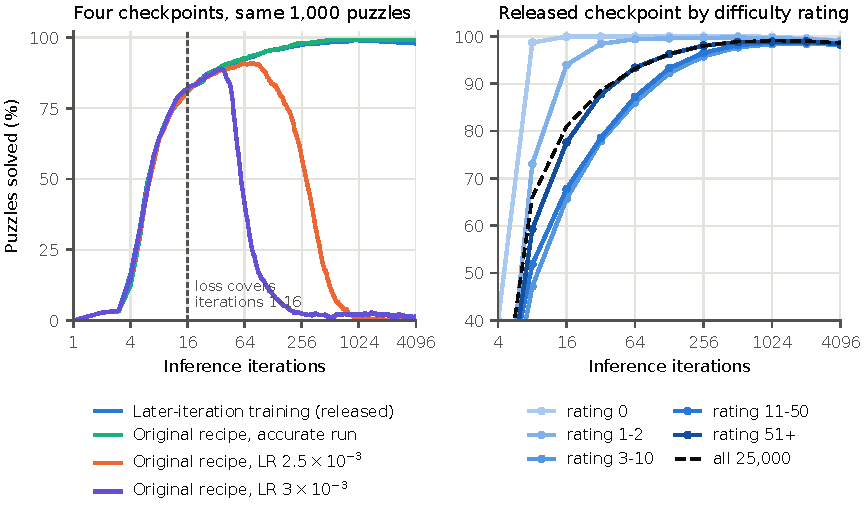
\includegraphics[width=0.92\linewidth]{iteration_scaling}
\caption{Accuracy as a function of the number of inference iterations, with FP32 inference. \emph{Left:} four checkpoints of the same architecture on the same 1,000 puzzles. All four were trained with the loss on at most 16 differentiable iterations, and all four solve about 81\% at 16 iterations. Two keep improving up to thousands of iterations; the other two, which differ from the accurate original run only in learning rate, lose almost everything. \emph{Right:} the released checkpoint on the 25,000-puzzle benchmark, by difficulty rating.}
\label{fig:scaling}
\end{figure}

\section{Model, training and evaluation}

Each of the 81 cells is a token, and the input $x$ is one-hot over ``empty'' and the nine digits. The model keeps a state $h_t\in\mathbb{R}^{81\times128}$ and reads digit probabilities $p_t$ off it after each iteration $t$:
\begin{align*}
h_0 = W_{\text{in}}\,x, \qquad p_0 = 0, \qquad
h_t = F\!\left(h_{t-1} + W_{\text{fb}}\,p_{t-1}\right), \qquad p_t = \operatorname{softmax}\!\left(W_{\text{out}}\,h_t\right).
\end{align*}
$F$ is a stack of four pre-norm transformer blocks (width 128, four heads, feed-forward width 512), for 796,937 parameters in total. The only position information is a 2D rotary embedding \citep{su2021roformer}, so the model knows the board is a grid and is told nothing about rows, columns or boxes. The puzzle goes in once, into $h_0$, and nothing normalizes the state between iterations.

The loss is cross-entropy on the empty cells, averaged over the predictions of 16 consecutive iterations. We use AdamW with learning rate \lr{2}, 1,400 warmup steps, cosine decay to 1\% of the peak, batch size 2048 and 50,000 steps in BF16 mixed precision (16-bit floats), on 2.7M puzzles of the Sudoku-Extreme training split \citep{wang2025hierarchical}, starting with the hardest puzzles and adding easier ones. We call this the \emph{original recipe}. A puzzle counts as solved only if every empty cell is filled correctly. Accuracy is measured on 25,000 test puzzles, 5,000 from each of five difficulty buckets, with FP32 inference. This benchmark guided our decisions for months, so it is really a development set (\autoref{sec:setup}).

\section{Results}

\paragraph{The accuracy came from ordinary choices.} At 16 iterations, training on the target dataset where we had used easier Kaggle puzzles, using more of it, a larger batch, learning-rate warmup and cosine decay took accuracy from 32\% to 84\% (\autoref{sec:history}). None of the fancier techniques we tried survived these basics. Sharpness-aware minimization \citep{foret2021sharpness} looked like our largest single gain (672 to 948 of 1,000 puzzles) until we fixed the learning-rate schedule, after which it was worth 0.4 points. The ingredients of the Tiny Recursive Model, a learned halting signal, the Muon optimizer and a network that is handed Sudoku's constraint graph didn't help either. Running the same weights for more iterations did: the released checkpoint solves 81\% at 16 iterations, 96\% at 128 and 99.1\% at 1024.

\paragraph{With the ordinary loss, it only works in some runs.} Our first four models all kept their accuracy at 1024 iterations. When we reran the two best configurations twelve times, two runs stayed above 90\% and nine fell below 6\%, with the same training loss and the same 81\% at 16 iterations (\autoref{sec:fragile}). The three original-recipe runs trained for this paper ended at 78.0\%, 2.5\% and 0.6\% (\tabref{tab:late}). Longer backpropagation, weight averaging, noise on the fed-back predictions, and losses that reward keeping a correct cell didn't change this.

\paragraph{Putting the loss on later iterations makes it dependable.} On 20\% of batches we first run $s$ iterations without gradients, with $s$ drawn from $\{32, 64, 128, 256, 512\}$, then detach the state and apply the same 16-iteration loss to iterations $s{+}1$ through $s{+}16$. The method is close to the progressive loss of \citet{bansal2022end}, with a much longer gradient-free prefix. All seven 50K-step runs trained this way finish between 97.5\% and 99.2\% at 1024 iterations (\tabref{tab:late}), at about 1.9 times the training time. It isn't a complete fix: two of the seven runs lose more than six points between 1024 and 4096 iterations (\autoref{sec:late}).

\begin{table}[t]
\centering
\small
\caption{Final checkpoints of 50K-step runs on the 25,000-puzzle benchmark, FP32 inference, accuracy (\%) by inference iterations. No checkpoint selection. The runs marked ``new'' were trained for this paper in a fresh environment, in pairs that share a seed.}
\label{tab:late}
\begin{tabular}{@{}llrrrrr@{}}
\toprule
Recipe & Seed & 16 & 128 & 1024 & 2048 & 4096 \\
\midrule
Later-iteration training (released) & 20260730 & 81.0 & 96.3 & 99.1 & 99.0 & 98.6 \\
Later-iteration training & 20260910 & 81.1 & 96.1 & 98.2 & 97.7 & 91.7 \\
Later-iteration training & 20260911 & 81.2 & 96.3 & 97.8 & 97.4 & 97.2 \\
Later-iteration training & 20260912 & 80.8 & 96.4 & 99.2 & 99.4 & 99.4 \\
\midrule
Later-iteration training (new) & 20261119 & 80.2 & 96.1 & 98.7 & 98.8 & 98.8 \\
Later-iteration training (new) & 20261120 & 81.2 & 96.0 & 97.5 & 95.2 & 83.9 \\
Later-iteration training (new) & 20261121 & 81.1 & 96.3 & 98.5 & 97.4 & 95.6 \\
\midrule
Original recipe (new) & 20261119 & 81.9 & 93.3 & 2.5 & 1.1 & 0.4 \\
Original recipe (new) & 20261120 & 81.6 & 94.1 & 78.0 & 73.0 & 68.4 \\
Original recipe (new) & 20261121 & 81.9 & 26.2 & 0.6 & 0.4 & 0.3 \\
\bottomrule
\end{tabular}
\end{table}%


\paragraph{The state never converges.} The state's magnitude grows linearly with the iteration count for as long as we have run it. For the released checkpoint the median root mean square is 393 at iteration 1024 and 1,730 at iteration 4096, while each update stays near 0.45. Predictions depend only on the state's direction. A model that keeps its answers stops changing direction. A model that loses them keeps drifting until a wrong digit overtakes the right one in some cell (\autoref{sec:analysis}).

\paragraph{Measure in adequate precision.} Running inference in BF16, as training does, lowers the released checkpoint from 98.6\% to 43.7\% at 4096 iterations, because the state grows until each iteration's update gets rounded away. Storing just the state in FP32 restores the FP32 result. We also withdrew a Jacobian analysis that was off by a factor of fifty, and found that 10K-step training runs ranked methods in the opposite order from 20K-step runs (\autoref{sec:pitfalls}).

\section{Limits and conclusion}
\label{sec:conclusion}

Everything here is about one task and one family of very small models, on a benchmark that we reused during development, and several comparisons rest on one to three runs. We don't know why the original recipe works in some runs and fails in others. With the full training split, a plain looped transformer went from 32\% to 99\% without any ingredient that is specific to it, and the one change it needed for reliability is a choice of the iterations that get the ordinary loss. A paper that proposes more machinery for this benchmark should include a plain loop that got the same number of tuning runs.

\paragraph{Acknowledgments.} AI coding assistants did a large share of the experiments, the analysis code and the drafting of this paper, under the author's direction. The author is responsible for the content.

\bibliographystyle{plainnat}
\bibliography{references}

\clearpage
\appendix
% The full account. sotaku_short.tex includes this file as the first part of its appendix.
\section{Setup}
\label{sec:setup}

\begin{table}[t]
\centering
\small
\caption{Reported results for looped transformers trained on the full Sudoku-Extreme training split, plus a feed-forward transformer for reference. Values marked $\approx$ were read off a plot. The setups differ in more than the model, so this is not a controlled comparison.}
\label{tab:baselines}
\begin{tabular}{@{}p{8.6cm}rrr@{}}
\toprule
Model & Parameters & Training puzzles & Solved (\%) \\
\midrule
Feed-forward transformer, 8 layers \citep{wang2025hierarchical} & 27M & 3.83M & 16.9 \\
``Recurrent Transformer'' baseline, best depth \citep{wang2025hierarchical} & not stated & 3.83M & $\approx$81 \\
Universal Transformer, one block, learned halting \citep{sapunov2026utmemory} & 3.2M & 3.83M & 2.5 \\
\quad with 8--32 added memory tokens & 3.2M & 3.83M & 57.4 \\
Looped denoiser, diffusion objective, attention limited to a cell's row, column and box \citep{drozdova2026diffusioncurriculum} & not checked & 3.83M & 99.9 \\
\quad the same model run without injected noise & & & 49.4 \\
Hierarchical Reasoning Model, deepest setting \citep{wang2025hierarchical} & 27M & 3.83M & $\approx$99 \\
\midrule
Sotaku (this paper), full test split, 1024 iterations & 0.8M & 2.7M & 98.94%
 \\
\bottomrule
\end{tabular}
\end{table}

\paragraph{Data and evaluation.} We use Sudoku-Extreme \citep{wang2025hierarchical}, where each puzzle is rated by the number of times a reference solver had to backtrack, and train on the first 2.7M puzzles of its training split. A puzzle counts as solved only if every empty cell is correct. Accuracy is the percentage of puzzles solved on a fixed benchmark of 25,000 test puzzles, 5,000 from each of five rating buckets (0, 1--2, 3--10, 11--50 and 51+), with inference in 32-bit floats (FP32). This benchmark guided our decisions for months, so it is really a development set. We also report the released checkpoint on all 422,786 test puzzles.

\paragraph{Model.} Each of the 81 cells is a token, and the input $x$ is one-hot over ``empty'' and the nine digits. The model keeps a state $h_t$, a vector of 128 numbers per cell, and after each iteration $t$ it reads digit probabilities $p_t$ off the state:
\begin{align*}
h_0 = W_{\text{in}}\,x, \qquad p_0 = 0, \qquad
h_t = F\!\left(h_{t-1} + W_{\text{fb}}\,p_{t-1}\right), \qquad p_t = \operatorname{softmax}\!\left(W_{\text{out}}\,h_t\right).
\end{align*}
$F$ is a stack of four ordinary pre-norm transformer blocks (width 128, four heads, 796,937 parameters in total), and one \emph{iteration} is one pass through $F$. The only position information is a 2D rotary embedding \citep{su2021roformer}, so the model knows where each cell is on the grid and is not told which cells constrain each other. The puzzle goes in once, into $h_0$, and nothing normalizes the state between iterations.

\paragraph{Training.} The loss is cross-entropy on the empty cells, averaged over the predictions of 16 consecutive iterations. We use AdamW \citep{loshchilov2019decoupled} with learning rate \lr{2}, warmup, cosine decay \citep{loshchilov2017sgdr}, batch size 2048 and 50,000 steps, in 16-bit mixed precision (BF16). Training starts on the hardest puzzles and adds easier ones as it goes. We call this the \emph{original recipe}, and \appref{app:hyper} has every setting. \emph{Later-iteration training} (\secref{sec:late}) only changes which 16 iterations get the loss on some batches. A run takes 3 to 5.5 hours on one NVIDIA H200.

\section{How we got to this model and recipe}
\label{sec:history}

The design came out of about two hundred small experiments, mostly single runs. The repository has the complete list (\appref{app:repo}), and \figref{fig:waterfall} shows the changes we kept.

\begin{figure}[t]
\centering
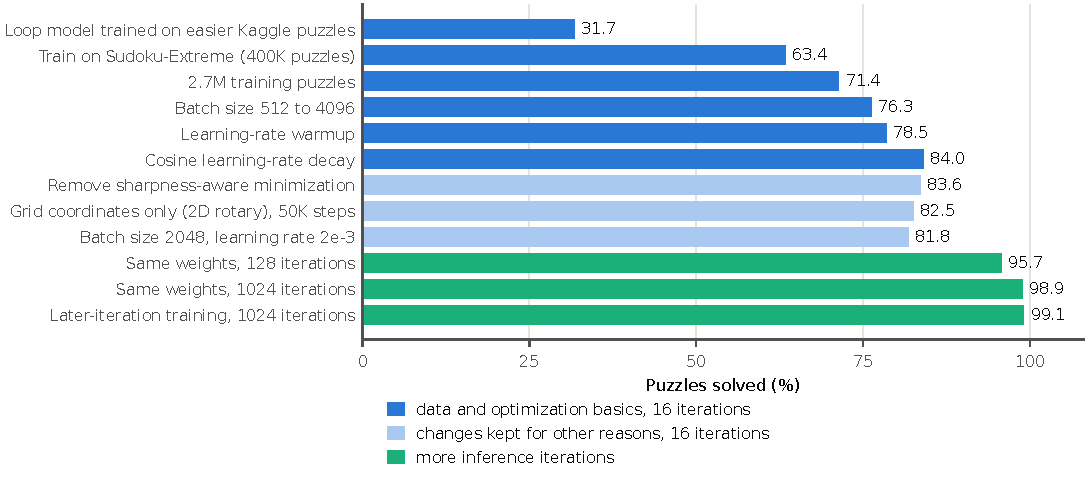
\includegraphics[width=0.86\linewidth]{where_accuracy_came_from}
\caption{Accuracy on Sudoku-Extreme after each change we kept, in order. Each bar is a single run with all earlier changes in place. The last three bars use the two published checkpoints.}
\label{fig:waterfall}
\end{figure}

\paragraph{Architecture.} The loop matters, and so does putting the loss on every iteration. On easy Kaggle puzzles \citep{radcliffe2020sudoku}, a model with 16 iterations solved 643 of 1,000 test puzzles, against none with one iteration and 428 with the loss on the last iteration only. Separate weights for each iteration did worse (581) with 16 times the parameters. The biggest architectural gain came from passing the hidden state from one iteration to the next along with the predicted probabilities. We started with learned row, column and box embeddings, which tell the model which cells constrain each other. Replacing them with 2D rotary embeddings cost only 0.3 points, and the model now works out rows, columns and boxes by itself (\secref{sec:analysis}).

\paragraph{Optimization.} A handful of ordinary changes took accuracy at 16 iterations from 32\% to 84\%: training on Sudoku-Extreme itself, more data, a larger batch, learning-rate warmup and cosine decay. Sharpness-aware minimization \citep{foret2021sharpness} is the result we would warn others about. Early on it looked essential, raising solved puzzles from 672 to 948 of 1,000. Once cosine decay was in, it was worth 0.4 points at twice the training cost, and we took it out.

\paragraph{Hard puzzles first.} Before cosine decay, the order in which the model saw difficulties mattered a lot: easy-to-hard solved 71.6\% of a mixed test set, uniform mixing 77.2\%, and hard-to-easy 79.8\%. With cosine decay, hard-to-easy and mixing ended up 0.2 points apart. We kept hard-to-easy.

\paragraph{What didn't help.} We tried most of the ingredients of the Tiny Recursive Model \citep{jolicoeur2025less,nanotrm}, the Muon optimizer \citep{jordan2024muon} and a learned halting signal. None improved on the plain model in our large-data setting. A recurrent relational network \citep{palm2018recurrent}, which is handed the graph of cells that constrain each other, did much worse. Nothing in \figref{fig:waterfall} is specific to Sudoku or to looped models.

\section{More iterations at inference, and why they only sometimes worked}
\label{sec:fragile}

So far every model was evaluated at the 16 iterations it was trained with. Running the same weights for longer costs only inference time, and accuracy kept climbing: our first published checkpoint improves at every doubling up to 1024 iterations and then holds (\tabref{tab:scaling}). Most puzzles don't need the extra iterations. Half of each rating bucket is solved within 9, while one in a hundred of the puzzles rated 3--50 needs more than 500. The rating also isn't quite what the model finds hard, since it solves puzzles rated 51+ faster than those rated 3--50. And progress on a hard puzzle isn't steady: in \figref{fig:board} the number of wrong cells goes down, back up, and down again.

\begin{table}[t]
\centering
\small
\caption{Accuracy (\%) by number of inference iterations, FP32. The first block uses the 25,000-puzzle benchmark; both checkpoints were trained with at most 16 differentiable iterations. The second block uses all 422,786 puzzles of the Sudoku-Extreme test split.}
\label{tab:scaling}
\setlength{\tabcolsep}{3.3pt}
\begin{tabular}{@{}lrrrrrrrrrrrrr@{}}
\toprule
Inference iterations & 1 & 2 & 4 & 8 & 16 & 32 & 64 & 128 & 256 & 512 & 1024 & 2048 & 4096 \\
\midrule
Released (later-iteration training) & 0.1 & 3.2 & 16.1 & 66.0 & 81.0 & 88.5 & 93.2 & 96.3 & 98.0 & 98.9 & 99.1 & 99.0 & 98.6 \\
Version 1 (original recipe) & 0.0 & 3.2 & 13.3 & 65.4 & 81.8 & 88.6 & 92.8 & 95.7 & 97.5 & 98.5 & 98.9 & 99.0 & 99.0 \\
\midrule
\multicolumn{14}{@{}l}{\emph{Released checkpoint by rating bucket}} \\
\quad rating 0 & 0.5 & 15.8 & 39.9 & 98.7 & 100.0 & 100.0 & 100.0 & 100.0 & 100.0 & 100.0 & 99.9 & 99.6 & 99.1 \\
\quad rating 1-2 & 0.0 & 0.0 & 3.9 & 73.1 & 94.0 & 98.4 & 99.4 & 99.6 & 99.7 & 99.8 & 99.6 & 99.5 & 99.0 \\
\quad rating 3-10 & 0.0 & 0.0 & 9.3 & 47.2 & 65.7 & 77.9 & 86.0 & 92.2 & 95.8 & 97.7 & 98.4 & 98.5 & 98.2 \\
\quad rating 11-50 & 0.0 & 0.0 & 16.9 & 51.9 & 67.8 & 78.6 & 87.2 & 93.3 & 96.6 & 98.2 & 98.7 & 98.7 & 98.4 \\
\quad rating 51+ & 0.0 & 0.0 & 10.3 & 59.4 & 77.6 & 87.8 & 93.4 & 96.3 & 98.1 & 98.8 & 98.9 & 98.9 & 98.3 \\
\midrule
\multicolumn{14}{@{}l}{\emph{Full test split}} \\
Released (later-iteration training) &  &  &  &  & 76.02 &  &  & 94.97 &  &  & 98.94 &  &  \\
Version 1 (original recipe) &  &  &  &  & 76.79 &  &  & 93.95 &  &  & 98.50 &  &  \\
\bottomrule
\end{tabular}
\end{table}%


\begin{figure}[t]
\centering
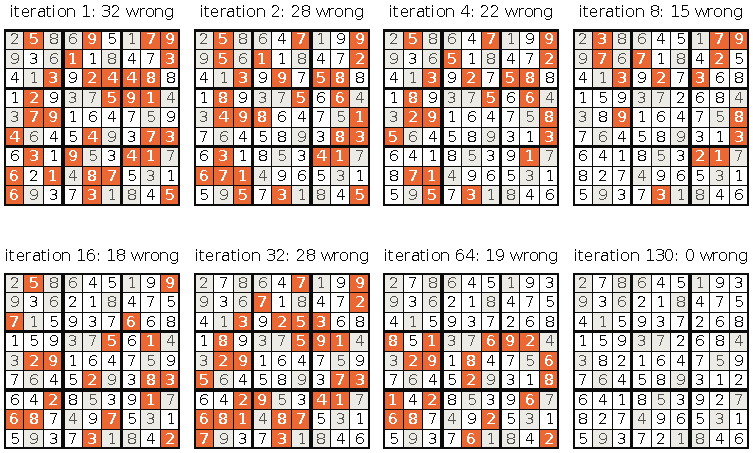
\includegraphics[width=0.72\linewidth]{board_evolution}
\caption{The released checkpoint's predictions for one puzzle rated 53. Grey cells are given and orange cells are wrong. The board has 15 wrong cells at iteration 8 and 28 at iteration 32. It is solved at iteration 130 and stays solved.}
\label{fig:board}
\end{figure}

\paragraph{The same recipe usually fails.} The four models we trained in February 2026 all kept their accuracy at 1024 iterations. In July, someone outside the project tried to reproduce the result and couldn't. We then reran the two best configurations twelve times. Two runs stayed above 90\% at 1024 iterations and nine fell below 6\%, although all twelve scored about 81\% at 16 iterations (\tabref{tab:repro}). We don't know why the first four runs all worked.

\begin{table}[t]
\centering
\small
\caption{Final checkpoints of every group of original-recipe runs. ``Kept'' counts runs with at least 90\% at 1024 iterations (80\% for the 20K-step monitoring group). The groups differ in schedule and inference precision, so the fractions shouldn't be pooled into one rate.}
\label{tab:repro}
\setlength{\tabcolsep}{4pt}
\begin{tabular}{@{}p{6.7cm}p{7.2cm}c@{}}
\toprule
Runs & Accuracy at 1024 iterations (\%) & Kept \\
\midrule
February, four configurations & 98.9, 98.1, 97.3, 95.9 & 4 of 4 \\
July, two best configurations rerun & 96.0, 92.3, 31.2, 5.8, 5.4, 3.0, 1.2, 0.2, 0.1, 0.1, 0.0, 0.0 & 2 of 12 \\
July, three-phase 40K-step variant & 24.6, 1.4, 0.3 & 0 of 3 \\
July, uniform difficulty mixing & 95.5, 88.8, 72.1 & 1 of 3 \\
July, eight more runs of the best configuration & 98.1, 97.1, and six lower & 2 of 8 \\
20K-step schedule, 1,000 monitoring puzzles & (threshold 80) & 2 of 7 \\
20K-step schedule, FP32 & 97.6, 11.0, 0.1 & 1 of 3 \\
50K steps, three new runs, FP32 (\secref{sec:late}) & 78.0, 2.5, 0.6 & 0 of 3 \\
\bottomrule
\end{tabular}
\end{table}

\paragraph{Accuracy at 1024 iterations swings during training.} With the original recipe, three checkpoints saved 1,000 steps apart in one run score 12.9\%, 97.3\% and 8.7\% at 1024 iterations, while the training loss and the 16-iteration accuracy change smoothly (\figref{fig:curves}). Picking the best checkpoint helps but isn't a fix.

\begin{figure}[t]
\centering
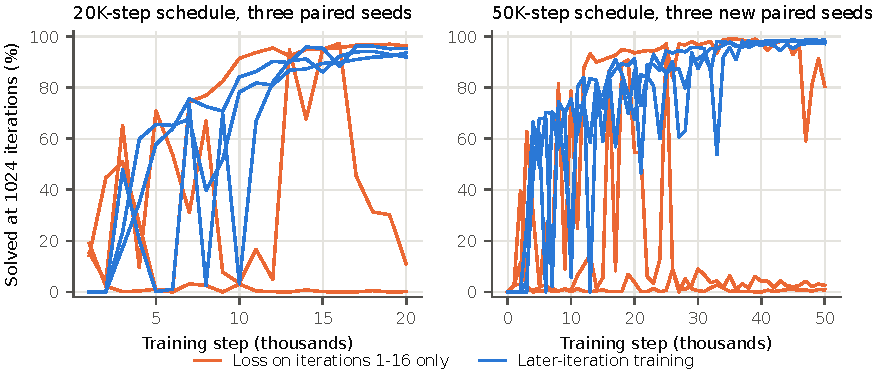
\includegraphics[width=\linewidth]{training_curves}
\caption{Accuracy at 1024 inference iterations during training, scored every 1,000 steps on 1,000 puzzles. Each line is one training run, and paired runs share a random seed.}
\label{fig:curves}
\end{figure}

\paragraph{What we tried that didn't change the odds.} Backpropagating through more iterations, with and without the residual scaling analyzed by \citet{wang2026loopmup}, averaging the weights, adding noise to the fed-back predictions, and adding losses that reward keeping a correct cell all left the failure as frequent or made it worse.

\section{Training on later iterations}
\label{sec:late}

\begin{figure}[t]
\centering
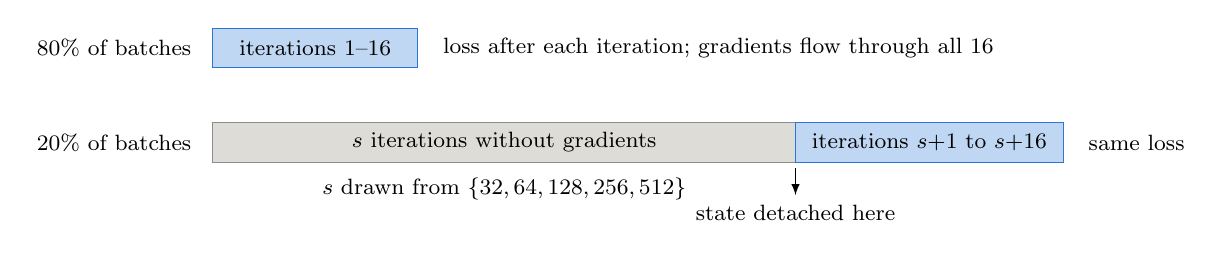
\begin{tikzpicture}[x=1cm,y=1cm,font=\footnotesize]
\definecolor{sup}{HTML}{2a78d6}
\definecolor{free}{HTML}{dddcd6}
\node[anchor=east] at (-0.15,1.45) {80\% of batches};
\draw[fill=sup!30,draw=sup] (0,1.2) rectangle (2.6,1.7);
\node at (1.3,1.45) {iterations 1--16};
\node[anchor=west] at (2.8,1.45) {loss after each iteration; gradients flow through all 16};
\node[anchor=east] at (-0.15,0.25) {20\% of batches};
\draw[fill=free,draw=black!45] (0,0) rectangle (7.4,0.5);
\node at (3.7,0.25) {$s$ iterations without gradients};
\draw[fill=sup!30,draw=sup] (7.4,0) rectangle (10.8,0.5);
\node at (9.1,0.25) {iterations $s{+}1$ to $s{+}16$};
\node[anchor=west] at (11.0,0.25) {same loss};
\draw[-{latex}] (7.4,-0.08) -- (7.4,-0.42);
\node[anchor=north] at (7.4,-0.42) {state detached here};
\node[anchor=north] at (3.7,-0.08) {$s$ drawn from $\{32, 64, 128, 256, 512\}$};
\end{tikzpicture}
\caption{Later-iteration training. On a random fifth of the batches, the 16 iterations that get the loss start from the state the model reaches after $s$ gradient-free iterations. Nothing else changes from the original recipe.}
\label{fig:method}
\end{figure}

The original recipe only ever puts the loss on the first 16 states of a trajectory. Our fix is to put it on later states too, without paying to backpropagate through the iterations that lead there (\figref{fig:method}). On 20\% of batches we draw $s$ from $\{32, 64, 128, 256, 512\}$, run $s$ iterations without gradients, detach the state, and apply the same 16-iteration loss to iterations $s{+}1$ through $s{+}16$. The other batches train as before. Training now reaches iteration 528 while gradients never span more than 16, and it takes about 1.9 times as long. This is a form of truncated backpropagation through time, close to the progressive loss of \citet{bansal2022end}. Ours uses a much longer gradient-free prefix and applies it to a minority of batches.

\paragraph{Results.} All seven 50K-step runs trained this way finish between 97.5\% and 99.2\% at 1024 iterations (\tabref{tab:late}). The last six rows of the table are three seed-matched pairs trained for this paper (\appref{app:cohort}). The original recipe ends at 2.5\%, 78.0\% and 0.6\%, and later-iteration training at 98.7\%, 97.5\% and 98.5\%. The later windows cost up to 1.7 points at 16 iterations. The released checkpoint comes from an earlier five-recipe comparison that agrees (\tabref{tab:matched} in \appref{app:ablations}).

\ifshort\else
\begin{table}[t]
\centering
\small
\caption{Final checkpoints of 50K-step runs on the 25,000-puzzle benchmark, FP32 inference, accuracy (\%) by inference iterations. No checkpoint selection. The runs marked ``new'' were trained for this paper in a fresh environment, in pairs that share a seed.}
\label{tab:late}
\begin{tabular}{@{}llrrrrr@{}}
\toprule
Recipe & Seed & 16 & 128 & 1024 & 2048 & 4096 \\
\midrule
Later-iteration training (released) & 20260730 & 81.0 & 96.3 & 99.1 & 99.0 & 98.6 \\
Later-iteration training & 20260910 & 81.1 & 96.1 & 98.2 & 97.7 & 91.7 \\
Later-iteration training & 20260911 & 81.2 & 96.3 & 97.8 & 97.4 & 97.2 \\
Later-iteration training & 20260912 & 80.8 & 96.4 & 99.2 & 99.4 & 99.4 \\
\midrule
Later-iteration training (new) & 20261119 & 80.2 & 96.1 & 98.7 & 98.8 & 98.8 \\
Later-iteration training (new) & 20261120 & 81.2 & 96.0 & 97.5 & 95.2 & 83.9 \\
Later-iteration training (new) & 20261121 & 81.1 & 96.3 & 98.5 & 97.4 & 95.6 \\
\midrule
Original recipe (new) & 20261119 & 81.9 & 93.3 & 2.5 & 1.1 & 0.4 \\
Original recipe (new) & 20261120 & 81.6 & 94.1 & 78.0 & 73.0 & 68.4 \\
Original recipe (new) & 20261121 & 81.9 & 26.2 & 0.6 & 0.4 & 0.3 \\
\bottomrule
\end{tabular}
\end{table}%

\fi

\paragraph{What changes in the model.} The model gets better at keeping answers it already has. In one run we switched later-iteration training on partway through. Within a thousand training steps, the share of puzzles solved at iteration 1024 that were still solved 16 iterations later went from 92.7\% to 99.8\%, and accuracy at 1024 iterations went from 62.0\% to 94.5\%.

\paragraph{Which parts matter.} We ran these variations with one to three seeds each, so only the big effects should be trusted (\appref{app:ablations}). The starting points need to cover a \emph{range}: always starting at one fixed iteration gave models that stopped near 90\%. They also have to \emph{reach far enough}: in a related variant, runs whose training never went past iteration 192 ended below 60\% at 1024 iterations. More isn't better, though. Later windows on half of the batches, or starting points up to 1024, cost more and didn't help consistently.

\paragraph{What it doesn't fix.} Two of the seven runs lose more than six points between 1024 and 4096 iterations (\appref{app:cohort}), and accuracy at 1024 iterations still dips until late in training (\figref{fig:curves}). A wider model helped: with width 160, all three runs stayed above 98.5\% at 4096 iterations.

\paragraph{Other things we tried.} Dividing each cell's state by its root mean square after every iteration made the original recipe dependable, but its accuracy stopped at about 92\%. The loop design of the Inkling 2 Mini language model \citep{inkling2mini,goodfire2026inkling} had the same effect. There, each iteration starts again from the puzzle and reads a gated summary of the previous iteration, and layers inside an iteration are connected by attention residuals \citep{kimi2026attnres}. In 20K-step runs, models built this way never lost a puzzle they had solved, but they stopped at about 84\%, against 95\% at 1024 iterations for the plain model trained the same way. Fine-tuning with evolution strategies \citep{salimans2017evolution}, which only need forward passes, repaired some failed checkpoints (e.g.\ from 5.4\% to 96.2\% at 1024 iterations) and did nothing for others. We also checked that the failures aren't a side effect of reusing the benchmark: on 10,000 newly generated puzzles from a different generator \citep{ostermiller_qqwing}, three original-recipe models scored 99.96\%, 3.8\% and 0.0\%.

\section{What the loop is doing}
\label{sec:analysis}

\begin{figure}[t]
\centering
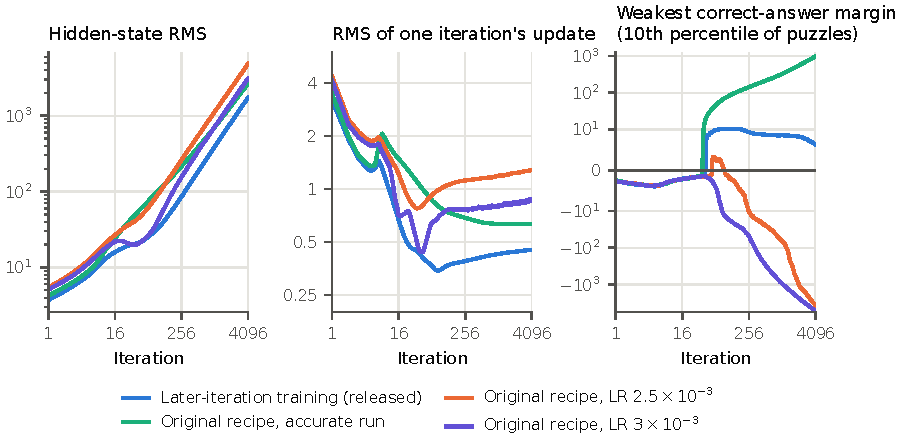
\includegraphics[width=\linewidth]{state_dynamics}
\caption{The state over 4,096 iterations for the four checkpoints of \figref{fig:scaling} (medians over 1,000 puzzles). \emph{Left:} the state's root mean square grows linearly in every model. \emph{Middle:} the size of one iteration's update levels off and doesn't shrink toward zero. \emph{Right:} for each puzzle we take the empty cell with the smallest gap between the correct digit's logit and the largest other logit, then show the 10th percentile across puzzles. Negative values mean a wrong digit is ahead in at least one cell.}
\label{fig:dynamics}
\end{figure}

\paragraph{There is no fixed point.} You might expect a model that holds its answer for thousands of iterations to have settled into a fixed point, where one more iteration changes nothing. That isn't what happens (\figref{fig:dynamics}). In every checkpoint we looked at, accurate or failing, the state's magnitude grows roughly linearly with the iteration count, and the size of each update levels off at a constant. Root-finding didn't find a useful solution of $F(h)=h$ either, so the model can't be treated as a deep equilibrium model \citep{bai2019deep} after the fact.

\paragraph{The answer is in the direction.} If we scale the state to length 1 and drop the output bias before reading the digits, accuracy stays within 0.3 points. So the answer is carried by the state's direction. An accurate model keeps pushing its state outward along a direction that has stopped changing: between iterations 896 and 1024 the direction moves by 0.006 in an accurate checkpoint and by 0.10 in a failing one.

\paragraph{Losing the answer is a slow drift.} In a failing checkpoint, the gap between the correct digit and its strongest competitor shrinks over hundreds of iterations until, in some cell, the competitor overtakes it (\figref{fig:dynamics}, right, and \figref{fig:timeline} in \appref{app:gallery}). The model has usually found the answer before that. In one failing model, 48 of 50 puzzles were solved at some iteration and only 2 were still solved at iteration 4096, and half of them ended on a wrong board that then stopped changing. The damage comes from the part of each update that is perpendicular to the state. Shrinking only that part to a quarter after iteration 128 brought three failing checkpoints back to about 95\% at 1024 iterations. This is only a diagnostic, and the released model runs unmodified.

\begin{figure}[t]
\centering
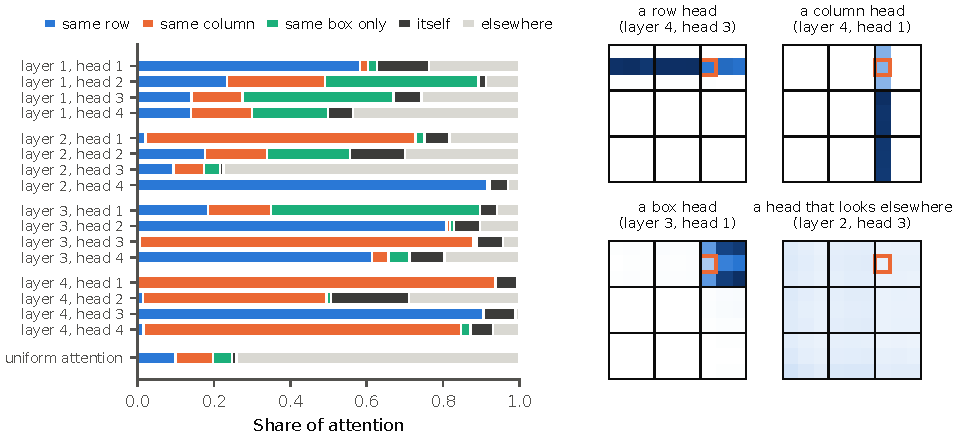
\includegraphics[width=0.95\linewidth]{attention_heads}
\caption{Attention in the released checkpoint at iteration 16, averaged over 1,000 puzzles. \emph{Left:} for each of the 16 heads, how attention from a cell is divided among the other cells of its row, of its column, the cells that share only its box, itself, and the remaining 60 cells. \emph{Right:} average attention from the outlined cell for four heads. The model is given row and column coordinates only, so it learned by itself to attend within the 3$\times$3 box.}
\label{fig:attention}
\end{figure}

\paragraph{Attention finds rows, columns and boxes.} The model gets each cell's row and column index and is told nothing about boxes. Most attention heads still specialize (\figref{fig:attention}, and \figref{fig:allheads} for all heads). Several put more than 80\% of their attention on the cell's row or on its column, and one puts 93\% inside the cell's 3$\times$3 box.

\paragraph{Nearby starts settle at different times.} Following \citet{lai2026fractal}, we nudged the starting state of a slowly solved puzzle along two random directions. The time it takes to settle changes in fine bands, down to nudges a thousand times smaller than the first ones (\figref{fig:maps}).

\paragraph{Compared with a hand-written solver.} A hand-written solver keeps a list of candidate digits for each cell and removes the candidates that clash with a filled cell in the same row, column or box. When that stalls, it guesses a digit and backtracks if the guess leads to a contradiction. It stops when the board is full, and its answer is correct by construction. The network has the first part: its attention heads read the same rows, columns and boxes that the elimination step reads, and a linear readout of its state recovers how many digits are still possible for a cell. The rest looks different. We see nothing like one guess being made and undone: on a hard puzzle many cells change in the same iteration, and the number of wrong cells goes up and down (\figref{fig:board}). The network finds different puzzles hard: the rating counts a solver's backtracks, yet the network solves the highest-rated puzzles faster than the middle ones. And it has no notion of being done. It never halts and nothing checks the board, so a failing model can settle on a wrong board and a correct board can be lost by running longer.

\section{Mistakes in measurement}
\label{sec:pitfalls}

\paragraph{Inference precision.} For most of the project, evaluation ran in BF16 mixed precision, the same as training. For the released checkpoint that lowers accuracy at 4096 iterations from 98.6\% to 43.7\% (\figref{fig:precision}, and \tabref{tab:precision} in \appref{app:precision}). A BF16 number keeps 8 significant bits. Once the state has grown to a few hundred while each update is still around 0.4, adding the update often rounds straight back to the old value. The fix is cheap: keep the BF16 arithmetic and store only the state passed between iterations in FP32. Precision doesn't explain the original recipe's failures, which also show up under FP32, but much of what we first believed about accuracy beyond 1024 iterations was really about rounding.

\begin{figure}[t]
\centering
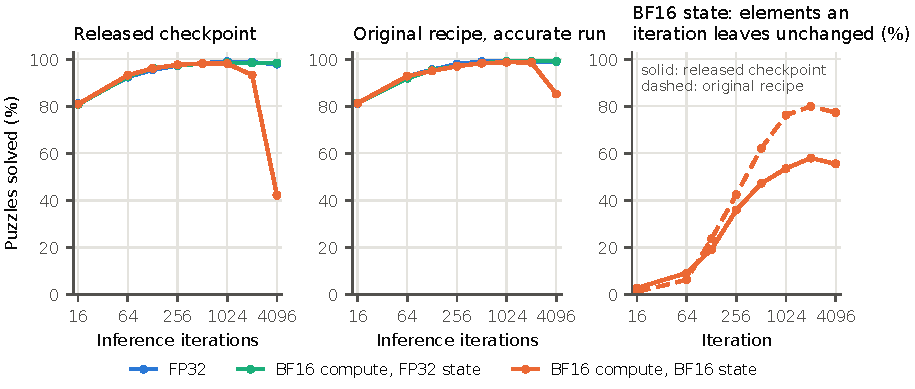
\includegraphics[width=\linewidth]{precision}
\caption{The same weights and the same 1,000 puzzles under three numerical settings. With BF16 arithmetic and a BF16 state, a growing share of state elements is left bit-for-bit unchanged by an iteration (\emph{right}), and accuracy at large iteration counts falls. With the same BF16 arithmetic and the state stored in FP32, accuracy matches full FP32.}
\label{fig:precision}
\end{figure}

\paragraph{A Jacobian that was off by fifty.} Our first stability analysis estimated the Jacobian of one iteration by finite differences in low precision. It reported spectral radii, a rough measure of whether small changes to the state grow, of 14 to 88, and we built explanations on top of it. Recomputed with automatic differentiation in FP64, the radius at the same state is 1.097, where the old method gave 52.5. We had been subtracting two nearly equal low-precision numbers and dividing by a small one. The corrected radius is about 1.1 in accurate and failing checkpoints alike, so it doesn't predict failure.

\paragraph{Shapes in projections.} Plot a state trajectory in its first principal components and you get clean lines, arcs and the occasional spiral (\figref{fig:pca} and \figref{fig:gallery} in \appref{app:gallery}). Number representations in language models are known to form helices \citep{kantamneni2025trigonometry}, so we went looking for one. The shapes changed with the projection and didn't repeat across puzzles, and random smooth paths with no Sudoku in them produced similar shapes once we picked the projection that maximized a helix score. A projection chosen after looking at the data isn't evidence of geometry.

\paragraph{Short runs and too few runs.} To save time we compared training variants with 10K-step runs. One variant finished far behind its control at 10K steps (20.5\% against 54.4\% at 1024 iterations) and ahead of it at 20K (94.8\% against 89.4\%). We now screen at 20K steps and confirm at 50K. The run-to-run variation of \secref{sec:fragile} went unnoticed for five months because the first four runs happened to succeed.

\section{Relation to prior work}
\label{sec:related}

\paragraph{What the project used.} We use the Sudoku-Extreme dataset released with the Hierarchical Reasoning Model \citep{wang2025hierarchical} and tested the ingredients of the Tiny Recursive Model \citep{jolicoeur2025less}. Both put the loss on several consecutive segments of a trajectory with the state detached between them, which is another way of training on later states. We also tried the residual scaling of \citet{wang2026loopmup} and the extra state of \citet{zeitoun2026hyperloop}, and neither removed the failure in our model. \citet{geiping2025scaling} train a looped language model with a truncation similar to ours.

\paragraph{What we found afterwards.} We searched the literature after the experiments were finished and haven't studied it in depth. The closest earlier method is the progressive loss of \citet{bansal2022end}, who also named the loss of accuracy at long iteration counts ``overthinking''. Their networks feed the input back in at every iteration and ours doesn't. The closest earlier architecture we know of is the recurrent transformer of \citet{yang2023learning}. Most later work on Sudoku-Extreme keeps the 1,000-puzzle setting, and several methods now report more than 99\% there \citep{huang2026eqr,chen2026ebr,hoover2026cram}, against about 50\% for our model (\appref{app:small}). \citet{chen2026ebr} report that their accuracy falls to 60\% when the energy-gradient update is replaced by a directly learned transition, while our result says that with the full training split a directly learned transition is enough. \citet{hoover2026cram} reach their accuracy with a classical energy trained in milliseconds and conclude that Sudoku shouldn't be used to test whether looped methods scale. We haven't reproduced these numbers.

\section{Hyperparameters}
\label{app:hyper}

\begin{table}[h]
\centering
\small
\caption{The released recipe. The original recipe is identical minus the ``later-iteration training'' block.}
\begin{tabular}{@{}p{4.6cm}p{10.9cm}@{}}
\toprule
\multicolumn{2}{@{}l}{\emph{Model}} \\
Tokens & 81 cells; input one-hot over 10 symbols; output 9 logits per cell \\
Blocks per iteration & 4, pre-norm, weights shared across iterations \\
Width, heads, feed-forward width & 128, 4, 512 (ReLU) \\
Position & 2D rotary embedding on queries and keys, 16 dimensions per axis, base 10 \\
Dropout & 0.1 (attention, residual branches, feed-forward) \\
State between iterations & previous state plus a linear map of the predicted probabilities; no normalization \\
Parameters & 796,937 \\
\midrule
\multicolumn{2}{@{}l}{\emph{Optimization}} \\
Loss & cross-entropy on empty cells, averaged over 16 iterations \\
Optimizer & AdamW, $\beta=(0.9, 0.95)$, weight decay 0.01, no gradient clipping \\
Learning rate & \lr{2} peak, 1,400-step linear warmup, cosine decay to 1\% of peak \\
Batch size, steps & 2048, 50,000 (20,000 with a 560-step warmup for the short schedule) \\
Precision & BF16 autocast with compiled model during training \\
Training pool & first 2.7M puzzles of the Sudoku-Extreme training split \\
Pool by step & rated 51+ (281K puzzles) to 10K; 11+ (1.64M) to 20K; 1+ (2.31M) to 30K; all to 50K \\
\midrule
\multicolumn{2}{@{}l}{\emph{Later-iteration training}} \\
Share of batches & 20\%, chosen independently per batch \\
Gradient-free iterations & drawn uniformly from $\{32, 64, 128, 256, 512\}$; dropout on \\
Loss & on the 16 iterations that follow, same loss; replaces the standard iterations 1--16 on those batches \\
\midrule
\multicolumn{2}{@{}l}{\emph{Inference}} \\
Precision & FP32, TensorFloat-32 disabled, batch size 256 \\
Iterations & 1024 unless stated; no early stopping, damping or answer selection \\
\bottomrule
\end{tabular}
\end{table}

\section{The six new training runs}
\label{app:cohort}

The six runs marked ``new'' in \tabref{tab:late} were trained on 19 November 2026 from the repository's unmodified code (PyTorch 2.10, one H200 GPU each), using three seeds fixed beforehand, with every started run reported.

\begin{table}[h]
\centering
\small
\caption{The six new runs. ``Best checkpoint'' and ``Final'' report FP32 accuracy (\%) at 1024 iterations on 1,000 benchmark puzzles across the 50 checkpoints saved every 1,000 steps. The last column counts how many of the 25,000 benchmark puzzles the final checkpoint solves at some iteration up to 4096 and later gets wrong.}
\label{tab:cohort}
\begin{tabular}{@{}llrrrr@{}}
\toprule
Recipe & Seed & Best checkpoint & at step & Final & Solved, then lost \\
\midrule
Later-iteration training & 20261119 & 98.7 & 45K & 98.6 & 166 \\
Later-iteration training & 20261120 & 98.2 & 37K & 97.4 & 4,155 \\
Later-iteration training & 20261121 & 98.5 & 42K & 97.2 & 950 \\
\midrule
Original recipe & 20261119 & 97.3 & 25K & 2.6 & 24,584 \\
Original recipe & 20261120 & 99.1 & 35K & 80.5 & 8,109 \\
Original recipe & 20261121 & 62.8 & 3K & 0.8 & 24,676 \\
\bottomrule
\end{tabular}
\end{table}

\paragraph{Checkpoint selection.} Selecting each original-recipe run's best checkpoint would yield 97.3\%, 99.1\%, and 62.8\%, against 2.6\%, 80.5\%, and 0.8\% for the final ones. With later-iteration training, the best checkpoint is within 1.3 points of the final one in every run.

\paragraph{The run that fades at 4096 iterations.} Later-iteration seed 20261120 drops from 97.5\% at 1024 iterations to 83.9\% at 4096, losing 11\% to 15\% of puzzles in every difficulty bucket including the easiest. Its state stays much smaller than in its sibling runs: at iteration 1024, median state RMS is 97 compared to 415 and 736. Meanwhile, the median margin in a puzzle's weakest cell erodes steadily from 15.5 logits at iteration 16 to 5.5 at 1024 and 2.0 at 4096, whereas the other two runs hold between 9 and 11. This looks like the drift analyzed in \secref{sec:analysis}, moving more slowly. We saw one such run and haven't tested whether wider starting offsets prevent it.

\section{Training on 1,000 puzzles}
\label{app:small}

HRM and TRM train on 1,000 puzzles expanded into 1,000 symmetry-augmented copies each, reporting 55.0\% and 87.4\% on the full test split \citep{wang2025hierarchical,jolicoeur2025less}. We ran our model in this regime, with relabeled digits, row and column permutations within and across bands, and random transposes as the augmentations.

\begin{table}[h]
\centering
\small
\caption{Our model trained on 1,000 puzzles: full-test-split accuracy (\%) in FP32. Multi-run rows report min--max across runs. The four runs in the second-to-last row span three seeds plus a second random sample of 1,000 puzzles.}
\label{tab:small}
\begin{tabular}{@{}lrlrrrrr@{}}
\toprule
 & & & & & \multicolumn{3}{c}{Inference iterations} \\
\cmidrule(l){6-8}
Difficulty sampling & Steps & Recipe & Weight decay & Runs & 16 & 128 & 1024 \\
\midrule
Hardest first & 50K & Original & 0.01 & 1 & 9.4 & 2.8 & 0.0 \\
Hardest first & 50K & Later-iteration & 0.01 & 1 & 13.0 & 14.1 & 10.6 \\
All from the start & 50K & Original & 0.01 & 1 & 20.9 & 16.4 & 0.0 \\
All from the start & 50K & Later-iteration & 0.01 & 1 & 22.7 & 22.0 & 18.9 \\
\midrule
All from the start & 10K & Original & 0.01 & 1 & 45.3 & 42.6 & 0.3 \\
All from the start & 10K & Original & 1.0 & 1 & 42.8 & 52.7 & 44.8 \\
All from the start & 10K & Later-iteration & 0.01 & 4 & 47.2--48.9 & 50.1--51.7 & 46.3--51.6 \\
All from the start & 10K & Later-iteration & 0.3 & 3 & 47.4--51.4 & 52.4--57.1 & 52.3--57.1 \\
\bottomrule
\end{tabular}
\end{table}

Left unmodified, both recipes memorize the 1,000 puzzles (\tabref{tab:small}). Sampling all difficulties from step 0 and cutting the schedule to 10,000 steps (a length we picked by inspecting test accuracy) recover most of the gap: later-iteration training then solves 46\% to 57\% at 1024 iterations across seven runs, matching HRM while trailing TRM by a wide margin.

\section{Additional figures}
\label{app:gallery}

\begin{figure}[H]
\centering
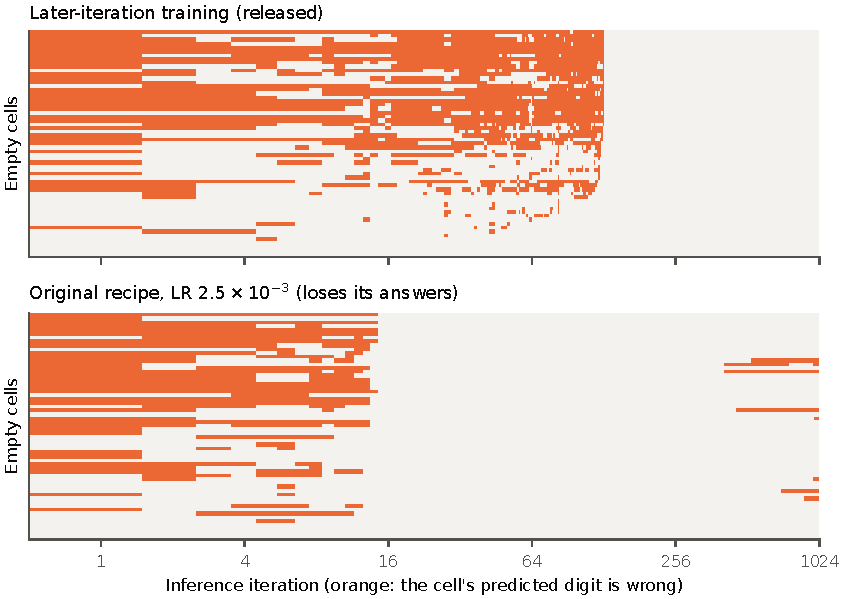
\includegraphics[width=0.76\linewidth]{cell_timeline}
\caption{The puzzle from \figref{fig:board} in two checkpoints. Each row is an empty cell, shaded orange on iterations where its prediction is wrong. \emph{Top:} the released checkpoint flips cells back and forth before solving the puzzle at iteration 130 and holding it. \emph{Bottom:} a failing original-recipe checkpoint solves the puzzle at iteration 15 and holds it until iteration 407, after which cells peel off one by one.}
\label{fig:timeline}
\end{figure}

\begin{figure}[H]
\centering
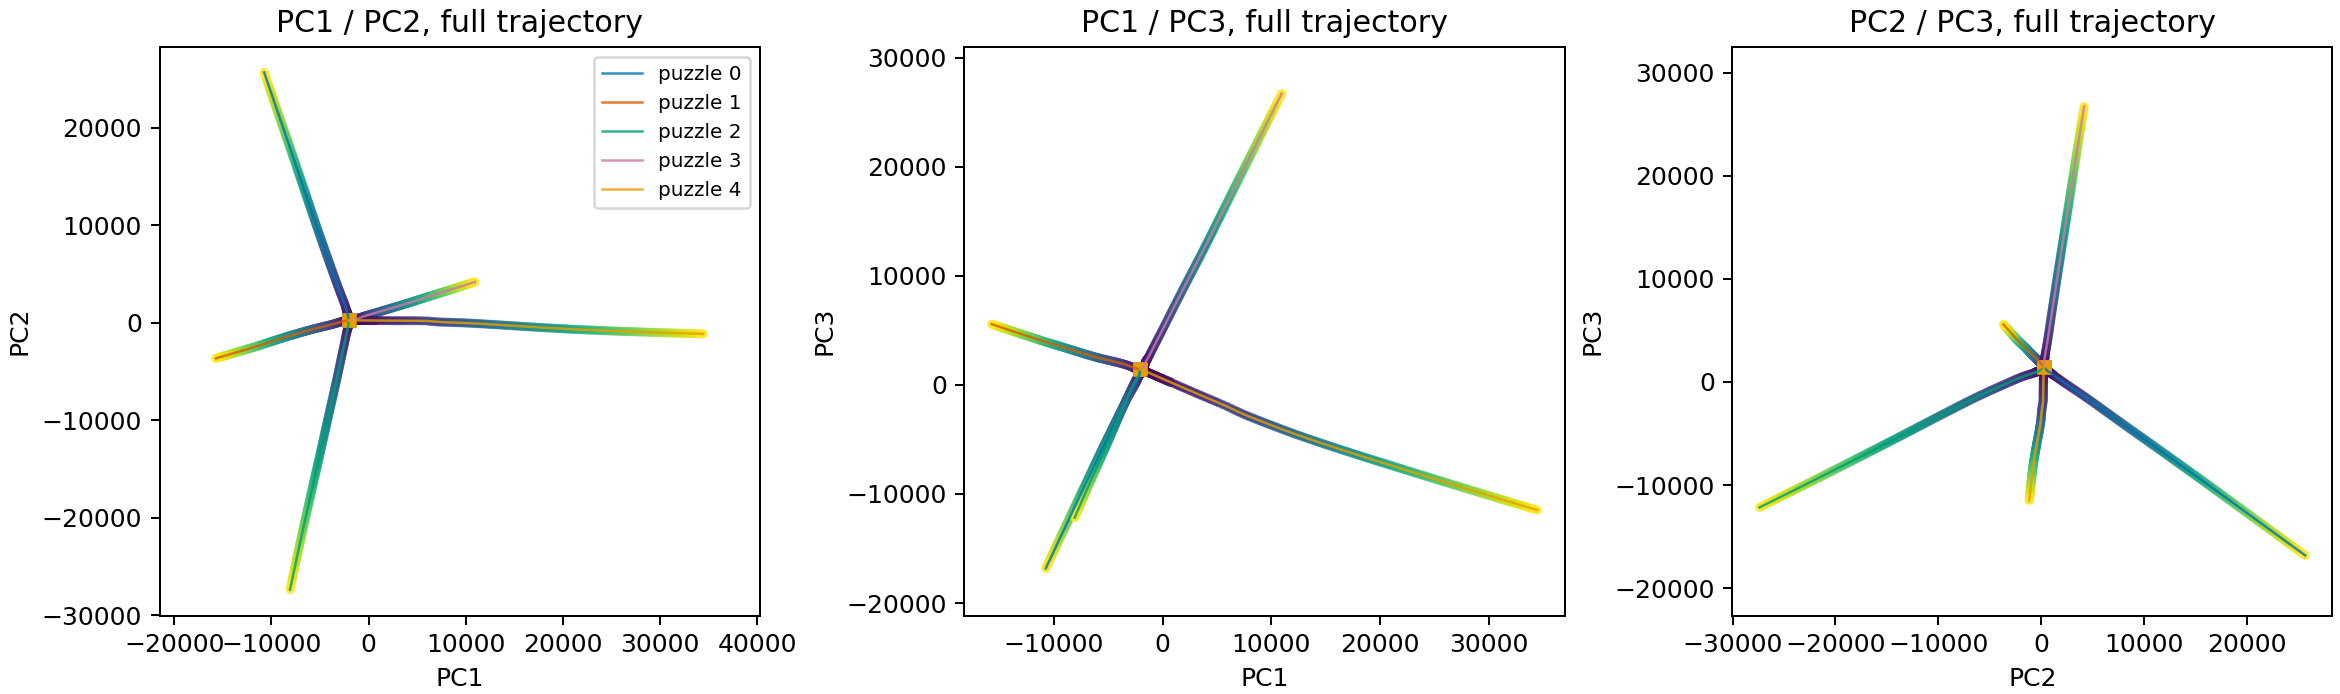
\includegraphics[width=\linewidth]{repo_state_pca}
\caption{State trajectories of five puzzles over 1,024 iterations in a shared PCA basis, colored from early (purple) to late (yellow), for a later-iteration checkpoint. Each puzzle traces a nearly straight ray corresponding to the linear norm growth in \secref{sec:analysis}.}
\label{fig:pca}
\end{figure}

\begin{figure}[H]
\centering
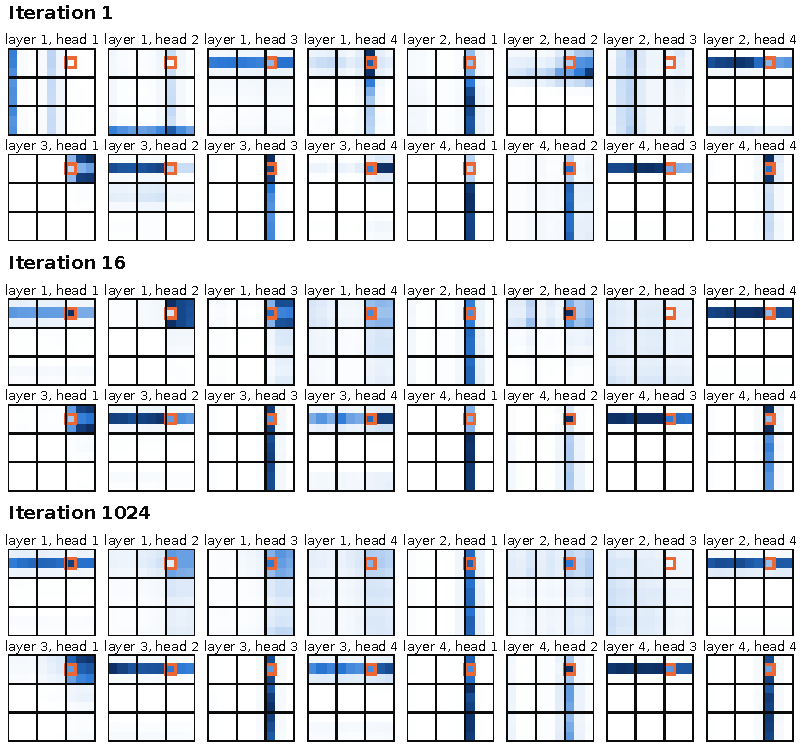
\includegraphics[width=\linewidth]{attention_all_heads}
\caption{All 16 attention heads of the released checkpoint at iterations 1, 16, and 1024. Each grid shows mean attention from the outlined cell over 1,000 puzzles on its own color scale. At iteration 1, several heads attend to rows or columns other than the cell's own. By iteration 16, the row, column, and box heads of \figref{fig:attention} have emerged, and they stay largely unchanged through iteration 1024.}
\label{fig:allheads}
\end{figure}

\begin{figure}[H]
\centering
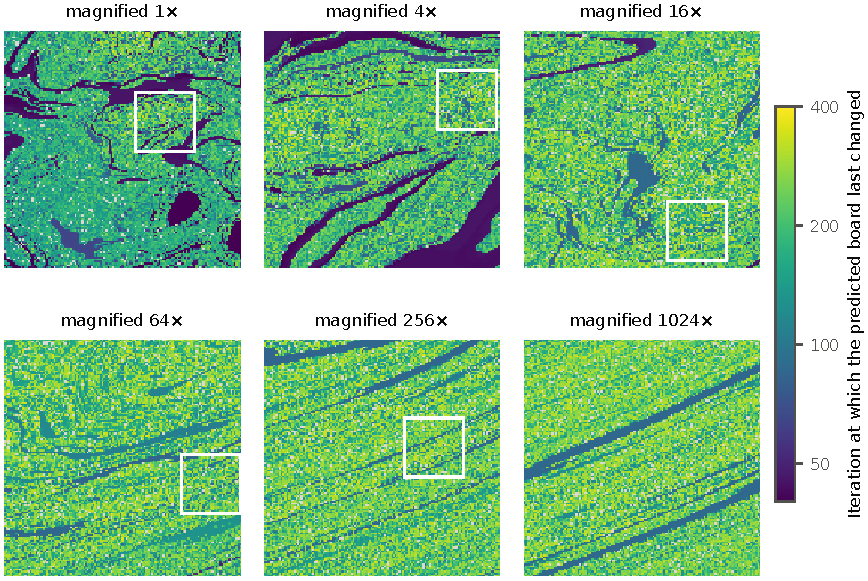
\includegraphics[width=0.88\linewidth]{perturbation_maps}
\caption{Nearby starting states can settle at very different iterations. Starting from a puzzle that an accurate 20K-step model solves slowly, we perturb $h_0$ along two random directions and run 2,048 FP64 iterations from a $129\times129$ grid of starts. Color marks the last iteration where the predicted board changed; grey marks the 2--6\% of starts that never landed on the right board. Each panel zooms into the white box of the previous one, and fine bands persist at $1,024\times$ magnification. For a puzzle solved in two iterations, the map is a single flat color.}
\label{fig:maps}
\end{figure}

\begin{figure}[H]
\centering
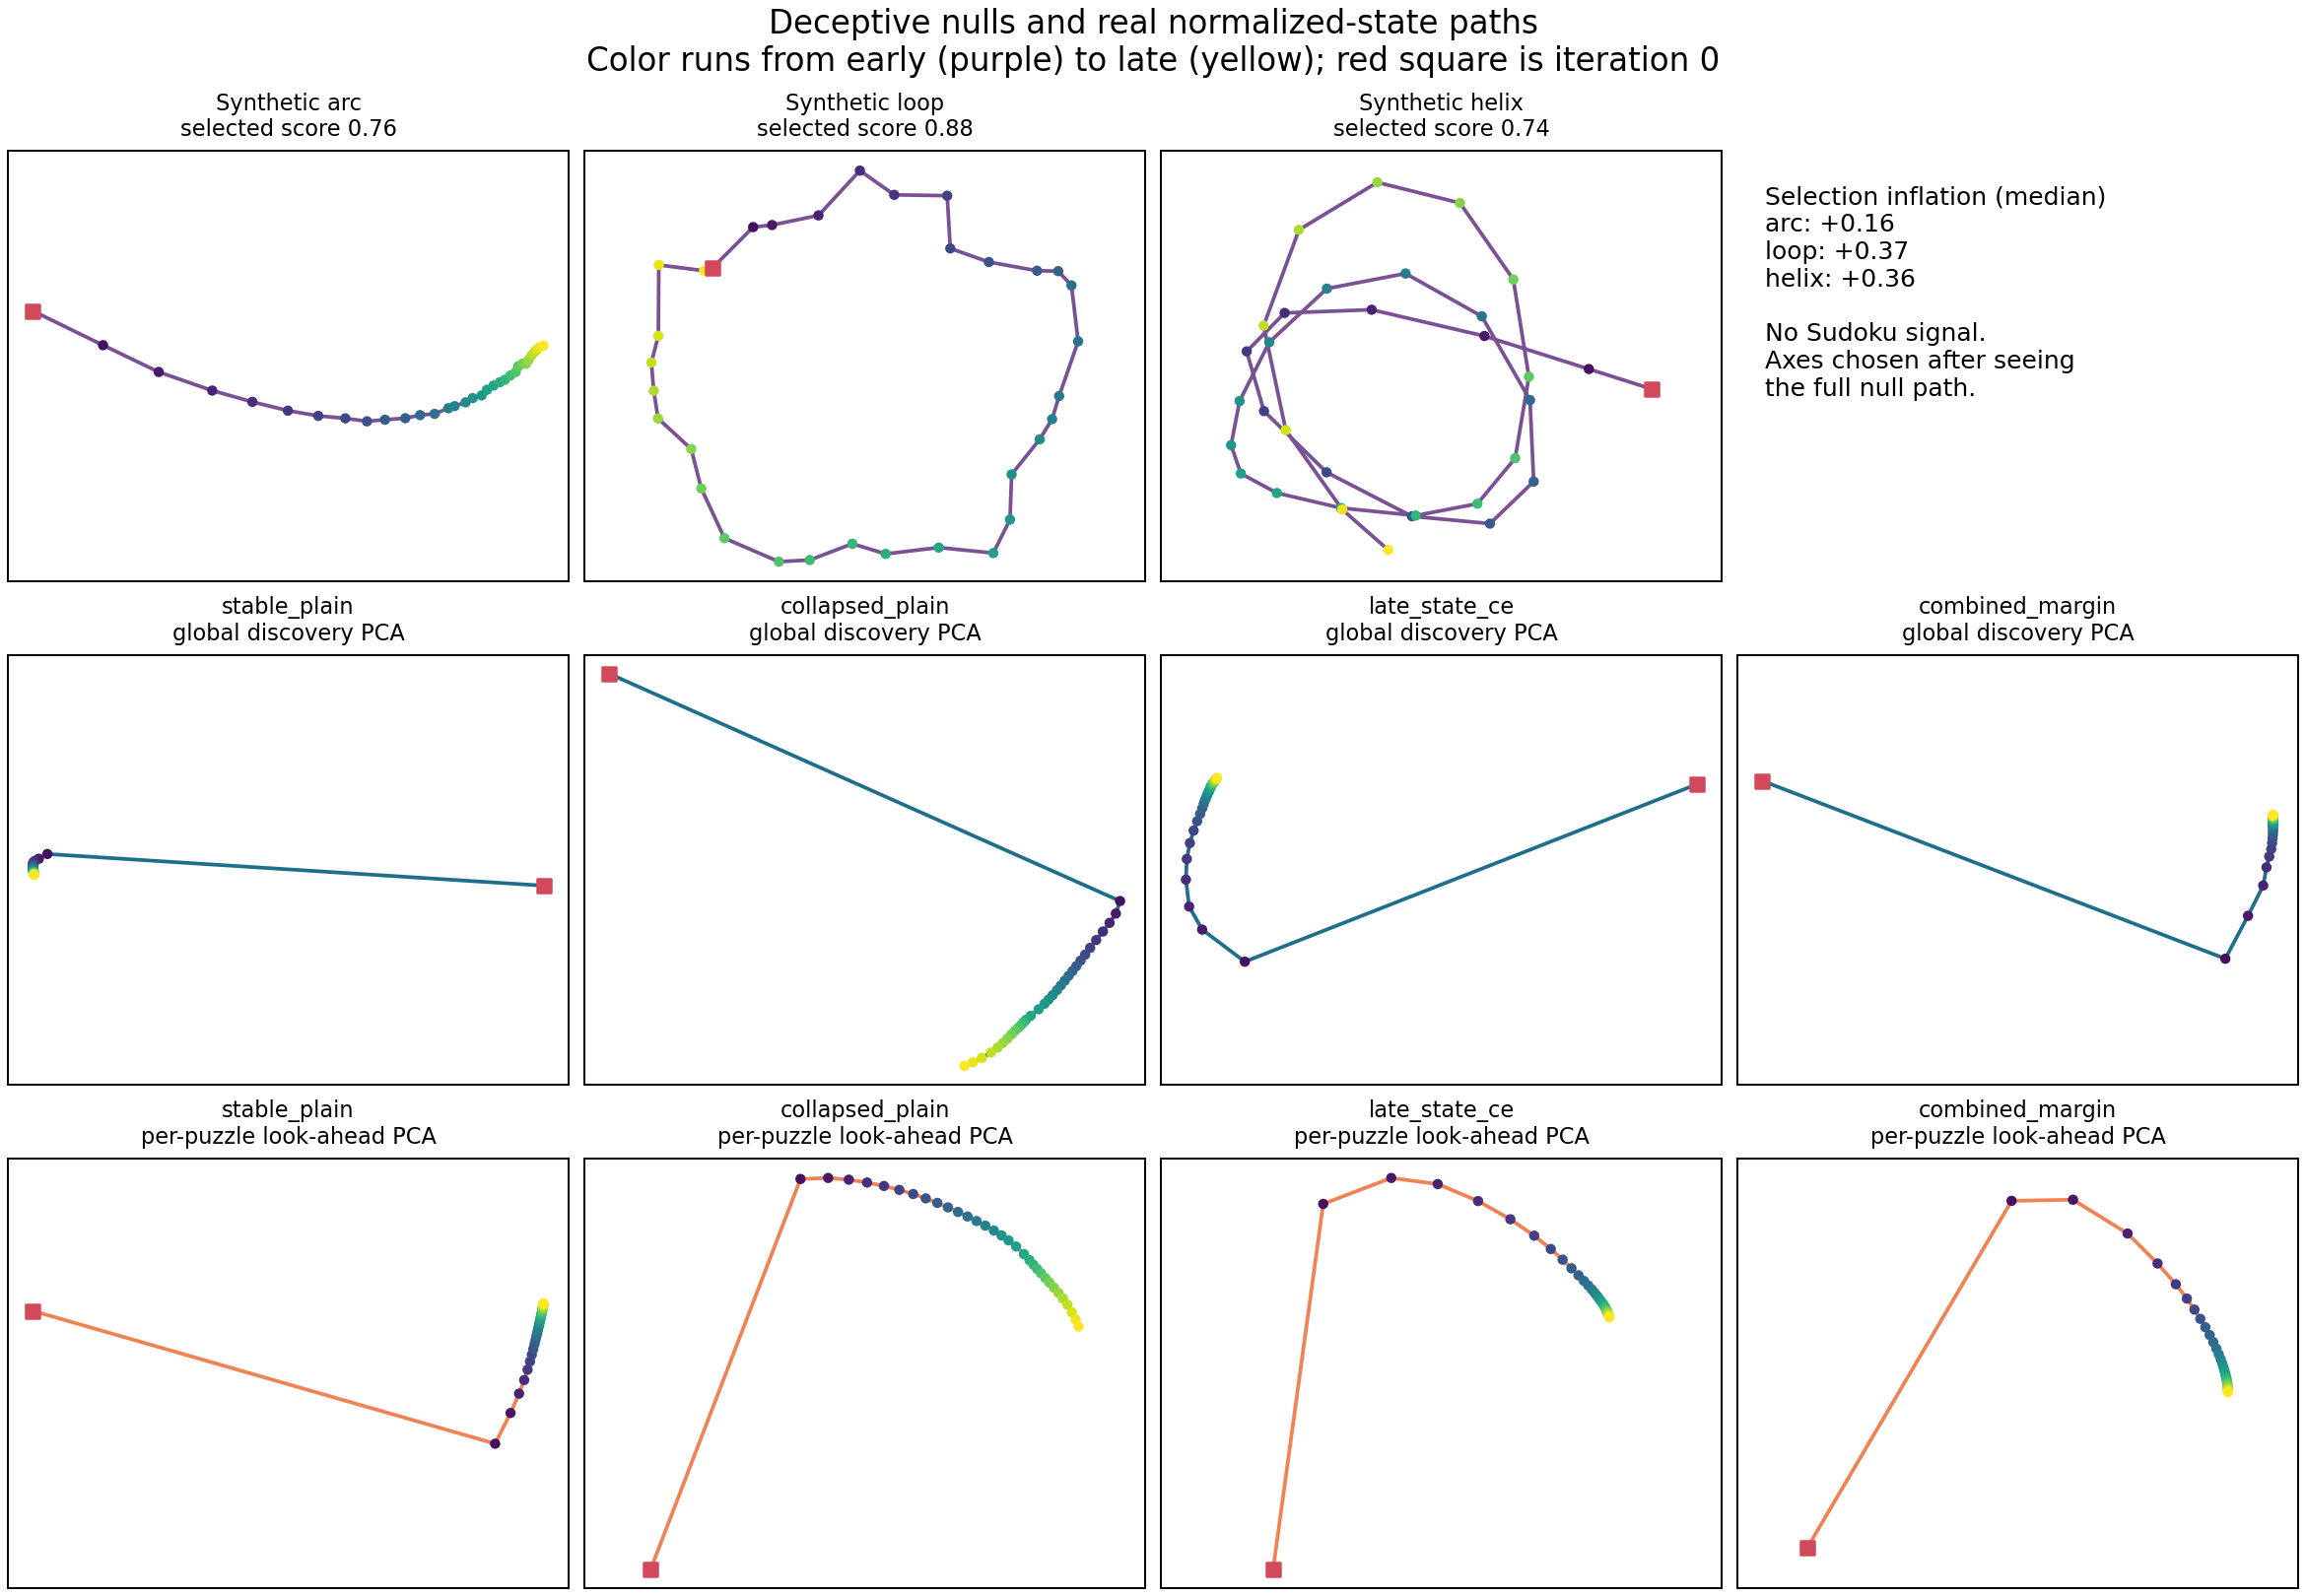
\includegraphics[width=0.70\linewidth]{repo_adversarial_gallery}
\caption{Why we stopped trusting trajectory projections. \emph{Top row:} random smooth curves with no Sudoku signal, each projected to maximize an arc, loop, or helix score. \emph{Other rows:} real trajectories, normalized to unit length, under a shared PCA basis and a per-puzzle basis. Labels use internal repository names: \texttt{stable\_plain} (accurate original-recipe checkpoint), \texttt{collapsed\_plain} (failing original-recipe checkpoint), \texttt{late\_state\_ce} (later-iteration training), and \texttt{combined\_margin} (adds a second window and late margin term).}
\label{fig:gallery}
\end{figure}

\section{Repository guide}
\label{app:repo}

The repository (\url{https://github.com/chenglou/sotaku}) contains full writeups for every experiment summarized here without a table; its README indexes them under ``Research Notes''. The main files are:

\begin{itemize}
\raggedright
\item \path{STALE_EXPERIMENTS_DOC.md}: the early design history in the order it happened, about two hundred experiments. \path{pos_embedding/EXPERIMENTS_POS.md}, \path{cosine/EXPERIMENTS_COSINE.md}, \path{muon/EXPERIMENTS_MUON.md} and \path{rrn/RRN_EXPERIMENTS.md} cover position encodings, the learning-rate schedule, Muon and the recurrent relational network.
\item \path{iters/EXPERIMENTS_ITERS.md}: accuracy at large iteration counts, the February and July runs, and the single runs with other learning rates, batch sizes and widths.
\item \path{looping/EXPERIMENTS_LOOPING.md}: later-iteration training, including the 20K-step runs, second windows, margin terms and damping at inference.
\item \path{stabilize/EXPERIMENTS_STABILIZE.md}: normalizing the state and the other attempts to stabilize the original recipe.
\item \path{es/EXPERIMENTS_ES.md}: evolution strategies, plus the pixel-input and maze variants of the task.
\item \path{looping/weight_tying/RESULTS.md}, \path{looping/window_selection/RESULTS.md}, \path{looping/width_50k/README.md}, \path{looping/hyperloop_50k/RESULTS.md} and \path{looping/attention_residuals/RESULTS.md}: shared against separate weights with the fresh puzzle set, the choice of starting points, width 160, the extra gated states, and the Inkling 2 Mini loop design.
\item \path{looping/trajectory_viz/study/README.md}, \path{looping/spectral_diagnostics/RESULTS.md} and \path{looping/basin_diagnostics/RESULTS.md}: the readout study and projection controls, the corrected Jacobian analysis, and the perturbation maps.
\item \path{release/PRECISION_RESULTS.md}: the inference-precision table. \path{paper/README.md}: how to rebuild this paper's tables and figures.
\end{itemize}


\end{document}
